\chapter{စက်ရုပ်ကားရဲလ် {\mycode{for}} Programming with Karel the Robot}
\XeTeXlinebreaklocale "my_MM"  %Myanmar line and character breaks
\XeTeXinterwordspaceshaping=2
\begin{sloppypar}
\enprogramming\ ဆိုတာဘာလဲ။ ဒါကိုဖြေဖို့ စာတွေအများကြီးရေးပြီး ရှင်းပြလို့ရပေမယ့် အများကြီးသိပ်မပြောပဲ လက်တွေ့ \enprogram လေးတွေ စရေးကြည့်ပြီးမှ \mmprogramming ဆိုတာ ဘာလဲ ပြောပြလိုက်ရင် ပိုပြီးနားလည်ရလွယ်တယ်။ ဒါ့ကြောင့် စက်ရုပ်ကားရဲလ်\myen{(Karel the Robot)}ကို အလုပ်တွေ လုပ်ခိုင်းဖို့ \mmprogram လေးတွေ  အရင်ဆုံး ရေးကြည့်ကြမယ်။

စက်ရုပ်ကားရဲလ်က အခြေခံအားဖြင့် \mycode{move, turnLeft, putBeeper, pickBeeper} ဆိုတဲ့ ကွန်မန်း\myen{(command)} လေးခုကို နားလည်တယ်။ \mycode{move} ကွန်မန်းက သူရပ်နေတဲ့ ကွန်နာ\myen{(corner)}ကနေ ရှေ့တည့်တည့် ကပ်ရပ် ကွန်နာဆီကို ရွှေ့ခိုင်းတာ။ \Fig \vref*{fig:name} မှာပြထားတဲ့ ကြက်ခြေခတ်လေးတွေကို ကွန်နာလို့ခေါ်တယ်။ 

\begin{figure}[!b]
    \centering\caption{ကားရဲလ်၏ {\mycode{for}} ကမ္ဘာ}\label{fig:name}
    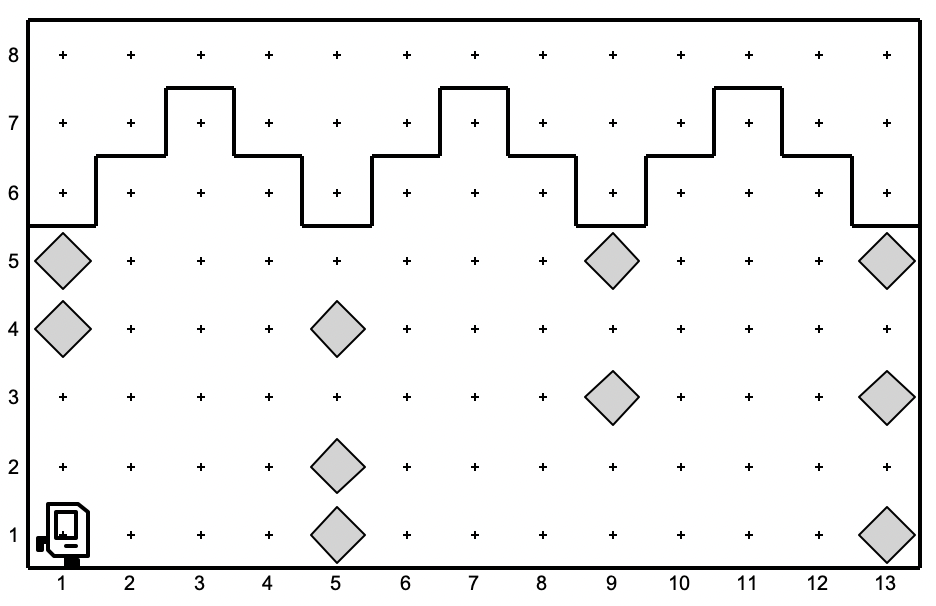
\includegraphics[width=4in]{ch01/ch01}
\end{figure}


\mycode{turnLeft} ကွန်မန်းကတော့ ဘယ်ဘက်လှည့်ခိုင်းတာ။ ကားရဲမျက်နှာမူရာ အရပ်မျက်နှာ တစ်ခုချင်းစီအတွက် \mycode{turnLeft} ကွန်မန်းပေးလိုက်တဲ့ အခါမှာ ဘယ်အရပ်ကိုလှည့်သွားမလဲ ပုံမှာတွေ့နိုင်တယ်။

ကားရဲလ်ကို \mycode{putBeeper} ကွန်မန်းပေးလိုက်ရင်တော့ ကားရဲလ်က သူရှိနေတဲ့ ကွန်နာမှာ ဘိပါ\myen{(beeper)} လို့ခေါ်တဲ့ အတုံးလေး တစ်ခုချထားလိမ့်မယ်။ ဒီကွန်မန်း မပေးရသေးခင်နဲ့ ပေးပြီးအခြေအနေကို ပုံမှာယှဉ်ပြထားတယ်။ ကွန်မန်းပေးပြီးသွားတဲ့အခါ စိန်တုံးပုံစံ ဘိပါတုံးလေး ရှိနေတာ တွေ့ရမယ်။ 

\mycode{pickBeeper} ကွန်မန်းက ဘိပါကောက်ခိုင်းတာပါ။ ကားရဲလ်ရောက်နေတဲ့ ကွန်နာမှာ ဘိပါရှိရင် ဒီကွန်မန်းနဲ့ ကောက်ခိုင်းလို့ရတယ်။ ကွန်နာတစ်ခုမှာ ဘိပါတစ်ခုမက ရှိနိုင်တယ်။ တစ်ခုမှ မရှိတာလဲ ဖြစ်နိုင်တယ်။ ပုံမှာဆိုရင် ကွန်နာတစ်ခုမှာပဲ ဘိပါရှိနေပြီး ကျန်တဲ့ ကွန်နာတွေမှာက ဘိပါမရှိပါဘူး။

ပရိုဂရမ်းမင်း\myen{(programming)} ဆိုတာဘာလဲ။ ဒါကိုဖြေဖို့ စာတွေအများကြီးရေးပြီး ရှင်းပြလို့ရသလို အများကြီးသိပ်မပြောပဲ လက်တွေ့ \myen{program} လေးတွေစရေးကြည့်ပြီးမှ ပရိုဂရမ်းမင်းဆိုတာ ဘာလဲ ပြောပြလိုက်ရင် ပိုပြီးနားလည်ရလွယ်တယ်။ ဒါ့ကြောင့် စက်ရုပ်ကားရဲလ်\myen{(Karel the Robot)}ကို အလုပ်တွေ လုပ်ခိုင်းဖို့ ပရိုဂရမ်\myen{(program)} လေးတွေ အရင်ဆုံး ရေးကြည့်ကြမယ်။

စက်ရုပ်ကားရဲလ်က အခြေခံအားဖြင့် \mycode{move, turnLeft, putBeeper, pickBeeper} ဆိုတဲ့ ကွန်မန်း\myen{(command)} လေးခုကို နားလည်တယ်။ \mycode{move} ကွန်မန်းက သူရပ်နေတဲ့ ကွန်နာ\myen{(corner)}ကနေ ရှေ့တည့်တည့် ကပ်ရပ် ကွန်နာဆီကို ရွှေ့ခိုင်းတာ။ ပုံမှာပြထားတဲ့ ကြက်ခြေခတ်လေးတွေကို ကွန်နာလို့ခေါ်တယ်။ 

\mycode{turnLeft} ကွန်မန်းကတော့ ဘယ်ဘက်လှည့်ခိုင်းတာ။ ကားရဲမျက်နှာမူရာ အရပ်မျက်နှာ တစ်ခုချင်းစီအတွက် \mycode{turnLeft} ကွန်မန်းပေးလိုက်တဲ့ အခါမှာ ဘယ်အရပ်ကိုလှည့်သွားမလဲ ပုံမှာတွေ့နိုင်တယ်။

ကားရဲလ်ကို \mycode{putBeeper} ကွန်မန်းပေးလိုက်ရင်တော့ ကားရဲလ်က သူရှိနေတဲ့ ကွန်နာမှာ ဘိပါ\myen{(beeper)} လို့ခေါ်တဲ့ အတုံးလေး တစ်ခုချထားလိမ့်မယ်။ ဒီကွန်မန်း မပေးရသေးခင်နဲ့ ပေးပြီးအခြေအနေကို ပုံမှာယှဉ်ပြထားတယ်။ ကွန်မန်းပေးပြီးသွားတဲ့အခါ စိန်တုံးပုံစံ ဘိပါတုံးလေး ရှိနေတာ တွေ့ရမယ်။ 

\mycode{pickBeeper} ကွန်မန်းက ဘိပါကောက်ခိုင်းတာပါ။ ကားရဲလ်ရောက်နေတဲ့ ကွန်နာမှာ ဘိပါရှိရင် ဒီကွန်မန်းနဲ့ ကောက်ခိုင်းလို့ရတယ်။ ကွန်နာတစ်ခုမှာ ဘိပါတစ်ခုမက ရှိနိုင်တယ်။ တစ်ခုမှ မရှိတာလဲ ဖြစ်နိုင်တယ်။ ပုံမှာဆိုရင် ကွန်နာတစ်ခုမှာပဲ ဘိပါရှိနေပြီး ကျန်တဲ့ ကွန်နာတွေမှာက ဘိပါမရှိပါဘူး။ \vref*{fig:name} မှာပြထားတဲ့ ကြက်ခြေခတ်လေးတွေကို ကွန်နာလို့ခေါ်တယ်။ 

ပရိုဂရမ်းမင်း\myen{(programming)} ဆိုတာဘာလဲ။ ဒါကိုဖြေဖို့ စာတွေအများကြီးရေးပြီး ရှင်းပြလို့ရသလို အများကြီးသိပ်မပြောပဲ လက်တွေ့ \myen{program} လေးတွေစရေးကြည့်ပြီးမှ ပရိုဂရမ်းမင်းဆိုတာ ဘာလဲ ပြောပြလိုက်ရင် ပိုပြီးနားလည်ရလွယ်တယ်။ ဒါ့ကြောင့် စက်ရုပ်ကားရဲလ်\myen{(Karel the Robot)}ကို အလုပ်တွေ လုပ်ခိုင်းဖို့ ပရိုဂရမ်\myen{(program)} လေးတွေ အရင်ဆုံး ရေးကြည့်ကြမယ်။

စက်ရုပ်ကားရဲလ်က အခြေခံအားဖြင့် \mycode{move, turnLeft, putBeeper, pickBeeper} ဆိုတဲ့ ကွန်မန်း\myen{(command)} လေးခုကို နားလည်တယ်။ \mycode{move} ကွန်မန်းက သူရပ်နေတဲ့ ကွန်နာ\myen{(corner)}ကနေ ရှေ့တည့်တည့် ကပ်ရပ် ကွန်နာဆီကို ရွှေ့ခိုင်းတာ။ ပုံမှာပြထားတဲ့ ကြက်ခြေခတ်လေးတွေကို ကွန်နာလို့ခေါ်တယ်။ 

\mycode{turnLeft} ကွန်မန်းကတော့ ဘယ်ဘက်လှည့်ခိုင်းတာ။ ကားရဲမျက်နှာမူရာ အရပ်မျက်နှာ တစ်ခုချင်းစီအတွက် \mycode{turnLeft} ကွန်မန်းပေးလိုက်တဲ့ အခါမှာ ဘယ်အရပ်ကိုလှည့်သွားမလဲ ပုံမှာတွေ့နိုင်တယ်။

ကားရဲလ်ကို \mycode{putBeeper} ကွန်မန်းပေးလိုက်ရင်တော့ ကားရဲလ်က သူရှိနေတဲ့ ကွန်နာမှာ ဘိပါ\myen{(beeper)} လို့ခေါ်တဲ့ အတုံးလေး တစ်ခုချထားလိမ့်မယ်။ ဒီကွန်မန်း မပေးရသေးခင်နဲ့ ပေးပြီးအခြေအနေကို ပုံမှာယှဉ်ပြထားတယ်။ ကွန်မန်းပေးပြီးသွားတဲ့အခါ စိန်တုံးပုံစံ ဘိပါတုံးလေး ရှိနေတာ တွေ့ရမယ်။ 

\mycode{pickBeeper} ကွန်မန်းက ဘိပါကောက်ခိုင်းတာပါ။ ကားရဲလ်ရောက်နေတဲ့ ကွန်နာမှာ ဘိပါရှိရင် ဒီကွန်မန်းနဲ့ ကောက်ခိုင်းလို့ရတယ်။ ကွန်နာတစ်ခုမှာ ဘိပါတစ်ခုမက ရှိနိုင်တယ်။ တစ်ခုမှ မရှိတာလဲ ဖြစ်နိုင်တယ်။ ပုံမှာဆိုရင် ကွန်နာတစ်ခုမှာပဲ ဘိပါရှိနေပြီး ကျန်တဲ့ ကွန်နာတွေမှာက ဘိပါမရှိပါဘူး။ \Fig\vref*{fig:name} မှာပြထားတဲ့ ကြက်ခြေခတ်လေးတွေကို ကွန်နာလို့ခေါ်တယ်။ 

\end{sloppypar}
